\part{Capítulo 10}
\section{Consideraciones generales}
\subsection{Tipos}
\begin{itemize}
    \item Cerámica:
    \begin{itemize}
        \item Ladrillos artesanales
        \item Ladrillos prensados: macizos, perforados o huecos
        \item Mampuestros: de muros, pisos o chimeneas
    \end{itemize}
    \item Hormigón:
    \begin{itemize}
        \item Bloques llenos
        \item Bloques huecos
    \end{itemize}
    \item Piedra:
    \begin{itemize}
        \item Sillarías: piedra labrada por todas sus Características
        \item Mampuestos: piedra labrada por una sola cara
        \item Piedra bruta: sin labrar
    \end{itemize}
    \item Adobe
\end{itemize}

La unión de piezas que formen una estructura se hace mediante mortero de cemento, logrando además:
\begin{itemize}
    \item Dar resistencia al muro
    \item Lograr un sellado entre juntas
    \item Adherencia con el acero de reguerzo en las juntas, los amarres metálicos y pernos de anclaje
    \item Dar una buena calidad arquitecónica
    \item Compensar las posibles variaciones de dimensiones de los bloques
\end{itemize}

\subsection{Albañilería de cerámicos o ladrillos de arcilla}
Materia prima del ladrillo cerámico es la arcilla, el agua, y en algunos casos aditivos especiales
Características:
\begin{itemize}
    \item Facilidad de uso tanto en soluciones constructivas simples como estructurales
    \item Propiedades mecánicas y físicas favorables, como:
    \begin{itemize}
        \item Permanencia: no hay procesos químicos que lo afecten, excepto ciclos de hielo y deshielo
        \item Resistencia a la compresión
        \item Buen aislante térmico y acústico
        \item Resistencia al fuego
        \item Buena adherencia con el mortero
        \item Buena integración con otros materiales
    \end{itemize}
    \item Gran variedad de calidades y de formas
    \item Confiere con facilidad textura superficial sin terminaciones ni revestimientos adicionales
\end{itemize}

\subsubsection{Ladrillos hechos a máquina}
Fabricado por amasado, moldeado y prensado de la pasta de arcilla
\begin{itemize}
    \item Extracción y transporte
    \item Preparación
    \item moldeadoCocción en horno
\end{itemize}
\subsubsection{Ladrillos hechos a mano}
\begin{itemize}
    \item Extracción de yacimientos de arcilla
    \item Preparación de la arcilla
    \item Mezcla de agua y arcilla
    \item Amasado
    \item Moldeado
    \item Secado
    \item Cocción
\end{itemize}

\subsection{Características y Propiedades de ladrillos de arcilla}
\begin{itemize}
    \item Resistencia a la compresión
    \item Absorción de agua
    \item Adherencia a cizalle
    \item Determinación de la eflorescencia
    \item Determinación de la succión
    \item Comprobación de dimensiones
    \item Comprobación de formas
    \item Desconchamientos
    \item Fisuras
\end{itemize}
\newpage
\subsubsection{Clasificación de ladrillos cerámicos}
\begin{itemize}
    \item Clasificación por uso
    \item Clasificación por clases
    \item Clasificación por grado
\end{itemize}

\begin{figure}
    \centering
    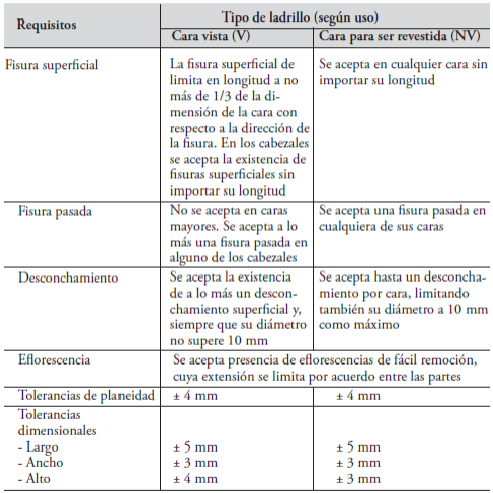
\includegraphics[width=0.5\textwidth]{FOTOS/clas_ladrillos_cer.png}
    \caption{Ladrillos}
    \label{fig:ladrillos}
\end{figure}

\begin{figure}
    \centering
    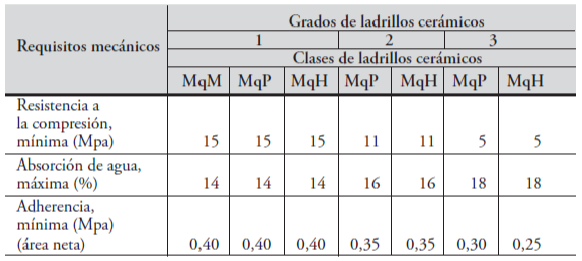
\includegraphics[width=0.5\textwidth]{FOTOS/clas_ladrillos_cer2.png}
    \caption{Ladrillos}
    \label{fig:ladrillos2}
\end{figure}

Existen tres tipos de Albañilería de ladrillo:
\begin{itemize}
    \item Albañilería simple o de relleno
    \item Albañilería armada
    \item Albañilería confinada
\end{itemize}

Muros de ladrillo:
\begin{itemize}
    \item Hilada
    \item Tendel o cantería
    \item Escantillado
\end{itemize}

\begin{figure}[h]
    \centering
    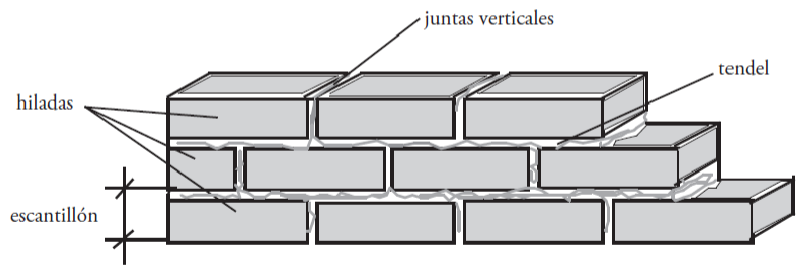
\includegraphics[width=0.5\textwidth]{FOTOS/muro_ladrillo.png}
    \caption{Muros de ladrillo}
    \label{fig:muros_ladrillo}
\end{figure}

Los aparejos más comunes son:
\begin{itemize}
    \item De Soga
    \item De Cabeza
    \item Pandereta
    \item De Sardinel
\end{itemize}

Algunas Consideraciones:
\begin{itemize}
    \item Tipo de aparejo a usar
    \item Traslapo de aparejos: se recomienda usar un traslapo de ½ si es ladrillo prensado y 1/3 si es ladrillo chonchón
\end{itemize}

Tipos de terminación del tendel o cantería:
\begin{itemize}
    \item Enrasado
    \item Rehundido
    \item Cóncavo
    \item En V
    \item Resaltado
    \item Matado (cortagotera)
\end{itemize}

Algunas Consideraciones:
\begin{itemize}
    \item Antes de colocar los ladrillos deben haber permanecido bajo agua durante 24 horas
    \item La primera hilada de ladrillos se pone de base y referencia
    \item Es necesario tener en cuenta la ubicación de vanos para puertas y ventanas
    \item Al poner las hiladas se debe conservar la altura del escantillón calculada previamente
    \item Hecha la albañilería, requiere curado que varía entre 3 y 15 días
    \item En caso de una albañilería armada, el diámetro del refuerzo vertical debe ser menor o igual a un medio de la menor dimensión del hueco en que irá inserto
    \item todos los huecos que llevan armadura de refuerzo deben llenarse con hormigón de relleno
\end{itemize}

\section{Inspección de obras}
Se eximen de los controles anteriores las viviendas individuales que cumplan simultáneamente las siguientes condiciones:
\begin{itemize}
    \item ener superficie inferior a 100 m2
    \item tener un número de pisos iguala o menor que dos
    \item ser construida bajo la supervisión directa del proyectista, quien calificará la calidad de la ejecución
    \item no formar parte de un conjunto de viviendas
\end{itemize}

\section{Albañilería de bloques de cemento}
Es más barata como solución constructiva que usando ladrillo de arcilla, pero no es más resistente
\begin{itemize}
    \item CLASE A: bloques para muros soportantes
    \item CLASE B: bloques para tabiques o muros no soportantes
\end{itemize}
La NCh 181 establece que para soporte se deben usar bloques de 190 mm o superior. Los de 140 mm se pueden usar para edificaciones de un piso o bien para divisiones interiores

\begin{itemize}
    \item Resistencia
    \item Absorción de humedad
    \item Aislación térmica
    \item Aislación acústica
    \item Resistencia al fuego
\end{itemize}

\subsection{Muros}
\begin{itemize}
    \item Albañilería simple
    \item Albañilería armada
    \item Albañilería confinada
\end{itemize}

\subsection{Consideraciones}
\begin{itemize}
    \item Mantener la verticalidad de los muros
    \item El mortero de junta debe estar fresco durante todo el tiempo de colocación
    \item La velocidad de elevación de una albañilería no debe exceder a 1.2 m. por día
    \item Las armaduras deben cumplir a las dimensiones especificadas y que no presenten óxido en escamas
    \item Todos los huecos que llevan armadura de refuerzo deben llevar hormigón de relleno
\end{itemize}

\subsection{Morteros para Albañilería}
\begin{itemize}
    \item mortero de junta
    \item mortero de relleno
    \item mortero de estuco
\end{itemize}